\documentclass[preprint,12pt]{elsarticle}

\usepackage{amssymb}
\usepackage{amsmath}
\IfFileExists{booktabs.sty}{\usepackage{booktabs}}{\newcommand{\toprule}{\hline}\newcommand{\midrule}{\hline}\newcommand{\bottomrule}{\hline}}
\usepackage{graphicx}
\usepackage{array}
\IfFileExists{lineno.sty}{\usepackage{lineno}}{\newcommand{\linenumbers}{}}
\usepackage{url}
\emergencystretch=2em

\journal{Biomedical Signal Processing and Control}

\begin{document}
\begin{frontmatter}

\title{From Identity Exposure to Selective Cross-Domain Calibration of Audit-Risk Probabilities in EEG Emotion Recognition}

\author[aff1]{Daohong Wei}
\ead{202311060931@std.uestc.edu.cn}
\author[aff2]{Tian Li}
\ead{202452080533@std.uestc.edu.cn}
\author[aff1]{Zhiqi Huang\corref{cor1}}
\ead{202121060701@std.uestc.edu.cn}
\author[aff3,aff1]{Dongyi Chen}
\ead{dychen@uestc.edu.cn}
\cortext[cor1]{Corresponding author.}

\affiliation[aff1]{organization={School of Automation Engineering, University of Electronic Science and Technology of China}, city={Chengdu}, postcode={611731}, country={China}}
\affiliation[aff2]{organization={School of Computer Science and Engineering, University of Electronic Science and Technology of China}, city={Chengdu}, postcode={611731}, country={China}}
\affiliation[aff3]{organization={School of Artificial Intelligence, Zhongyuan University of Technology}, city={Zhengzhou}, postcode={450007}, country={China}}

\begin{abstract}
Repeated-measures affective datasets can make classifiers appear deployable when participant identity overlaps training and test data. Split comparisons and identity probes indicate association or decodability, but neither isolates classifier utilization nor predicts material optimism.

We introduce a three-stage framework linking mechanism, risk, and cross-domain calibration. First, a counterfactual identity-dose experiment varies identity--label opportunity while fixing test rows, training size, class counts, and identity coverage. Second, an L2-logistic model uses five mechanism-derived predictors to estimate the probability that a configuration exhibits at least 0.02 balanced-accuracy optimism. Across the two leave-dataset-out public-source development tests, minimum AUROC and Brier skill were 0.698 and 0.100. On EPPVR, ranking transferred (AUROC 0.666), but calibration and the frozen operating point failed.

Third, Distribution-Covered Stratified Order-Preserving Calibration Transport (DCS-OPCT) applies a positive-slope CORAL probability map only when a complementary quantile witness agrees and a distribution-covered audit certifies Brier improvement. The original transductive outcome-held-out analysis released correction for EPPVR, CASE, and CEAP. In a stricter sensitivity that hid held-out covariates before assignment and transform fitting, EPPVR and CASE retained positive Brier gains, whereas CEAP reverted to the original probability. When endpoints were additionally reconstructed from disjoint raw test groups, only EPPVR remained certified, with gain 0.0135. A final EPPVR sensitivity split all 30 participants into two outcome-blind 15-person populations and independently rebuilt every dose experiment, identity probe, and emotion model (9,600 fits). Both audit-fitted component shifts exceeded the frozen 0.10 applicability limit, so the method returned the original probability before evaluation-population outcomes were used. A crossed bootstrap also showed that the binary 0.02 endpoint was measurement-uncertain; nevertheless, the EPPVR and CASE inductive actions retained positive soft-label gains. Across repeated matched-budget audits, no released DCS-OPCT action met the material-negative criterion, although finite-sample upper bounds remained nonzero and competing low-label calibrators sometimes released harmful actions.

DCS-OPCT therefore targets selective low-label intervention control, not superiority when target labels are abundant. It calibrates a configuration-level audit-risk probability, not EEG emotion predictions. Positive transport evidence remains retrospective and conditional on the evaluated target batch. In a prospectively reserved EKM-ED attempt locked before participant-value access, only 86 of 188 participant--film units satisfied the frozen three-window construction and no participant met the three-trial, both-class endpoint gate; execution therefore stopped before model fitting. This prospective structural failure and the fully training-row-disjoint EPPVR sensitivity support fail-closed protocol execution, but not calibration effectiveness. The study does not establish prospective external effectiveness, workflow-level audit utility, or future-domain non-harm.
\end{abstract}

\begin{highlights}
\item Counterfactual identity dose separates opportunity, encoding, and utilization.
\item Identity exposure can reverse model ranking under joint-unseen deployment.
\item A mechanism-derived audit-risk score transfers ranking but may lose calibration.
\item DCS-OPCT preserves ordering and releases only after a stratified audit certificate.
\item Stronger data separation contracts release and triggers fail-closed non-intervention.
\end{highlights}

\begin{keyword}
EEG emotion recognition \sep identity leakage \sep dataset shift \sep probability calibration \sep selective prediction \sep domain adaptation \sep audit risk
\end{keyword}
\end{frontmatter}

\linenumbers

\section{Introduction}
\label{sec:introduction}

Repeated-measures electroencephalography (EEG) datasets are central to affective-computing research \cite{alarcao2019survey,suhaimi2020review}. In DEAP and MAHNOB-HCI, each participant contributes responses to multiple audiovisual stimuli, allowing controlled comparison of features and models \cite{koelstra2012deap,soleymani2012mahnob}. The same design creates a recurring evaluation ambiguity: observations in a test set may come from participants whose other trials occur in training. If the split unit does not match the deployment unit, nominally held-out observations can remain statistically dependent on training data, and performance can reflect stable participant structure rather than a transferable physiology--affect relation \cite{kaufman2012leakage,roberts2017crossvalidation,saeb2017usecase,delpup2025partitioning}. Subject-dependent performance is useful for personalized systems, but it is not evidence of performance for a new user.

This issue is commonly addressed through subject-disjoint evaluation or subject-invariant representation learning \cite{rayatdoost2021subject,shen2023contrastive}. More broadly, shortcut learning describes predictive behavior that succeeds under the development distribution by exploiting an easier unintended signal \cite{geirhos2020shortcut}. Yet a comparison between overlapping and disjoint splits is not a controlled estimate of identity utilization: test composition, training size, class balance, and the set of available identities may all change together. An identity probe answers a different question. Above-chance subject prediction demonstrates that identity is encoded in the representation, but not that the emotion classifier uses it. A metadata-only identity prior shows label opportunity, but opportunity also need not be utilized. Treating split gaps, decodability, and utilization as interchangeable can therefore produce both false alarms and false reassurance.

The practical consequence extends beyond a biased headline accuracy. Evaluation is used to choose representations, model families, and hyperparameters. If identity exposure benefits candidates differently, the winner under an exposed protocol can differ from the winner under the intended new-subject, new-stimulus deployment condition. The resulting ranking reversal creates a measurable deployment regret. A useful audit therefore has to progress from detecting identity information to estimating whether identity opportunity materially changes performance and model selection.

Even a successful audit-risk model faces a second transfer problem. A score trained on one set of datasets may retain discrimination in a new domain while losing absolute probability calibration. This distinction is well established in probabilistic prediction: ranking metrics and proper scoring rules measure different properties, calibration itself requires explicit evaluation, and dataset shift can degrade probability reliability even when discrimination remains useful \cite{niculescu2005probabilities,guo2017calibration,vaicenavicius2019calibration,ovadia2019trust,minderer2021calibration}. Unsupervised alignment such as CORAL can reduce second-order feature discrepancy \cite{sun2016coral}. CPCS and TransCal further show that calibration can be transferred under covariate shift or domain adaptation assumptions \cite{park2020cpcs,wang2020transcal,pampari2020unsupervised}; however, unconditional correction may itself cause negative transfer when the target lies outside the support in which the transform was developed \cite{bendavid2010domains,ericsson2023better}.

Several neighboring method families solve related but different decisions. CPCS and TransCal calibrate instance-level classifier confidence under covariate-shift or domain-adaptation assumptions \cite{park2020cpcs,wang2020transcal}. Average-thresholded confidence estimates aggregate target accuracy without target labels \cite{garg2022atc}. Selective classifiers reject individual predictions \cite{geifman2019selectivenet}, whereas risk-controlling and conformal procedures certify a specified predictive risk under their calibration and distributional conditions \cite{bates2021risk,angelopoulos2024crc}. Table~\ref{tab:capability-matrix} makes the narrower capability claim explicit: DCS-OPCT is not presented as a new alignment, logistic-calibration, or certification primitive. Its contribution is to connect a counterfactual configuration-level shortcut endpoint to a domain-level applicability decision, a limited-label release certificate, verified order preservation, and an explicit return-original action.

We address these two transfer levels as one closed-loop engineering problem. Stage I constructs a counterfactual identity-dose experiment that varies identity--label opportunity while fixing the tested observations and matched training constraints. Stage II converts material dose-induced optimism into a configuration-level event and learns a frozen audit-risk model from mechanism-derived, dataset-agnostic predictors. Stage III introduces Distribution-Covered Stratified Order-Preserving Calibration Transport (DCS-OPCT), which corrects target-domain audit-risk probabilities only when two separately constructed unlabeled transformations agree and a fixed labeled audit certifies improvement. Otherwise, the method returns the original probability.

The study contributes four testable capabilities. First, the identity-dose intervention estimates utilization under a matched evaluation-protocol intervention rather than inferring use from opportunity or decodability. Second, the consequence analysis links that utilization to winner reversal, pairwise rank inversion, and joint-unseen regret. Third, the frozen risk model predicts a configuration-level material-optimism event without dataset, task, representation, or model identities as predictors. Fourth, DCS-OPCT couples a separately constructed applicability screen, an order-preserving candidate, an outcome-blind audit, and a limited-label release certificate. Matched-budget comparisons separate this complete decision path from direct calibration, label splitting, and out-of-fold certification. The bounded empirical claim follows an explicit independence ladder: three corrections were supported under transductive outcome holdout, two remained supported when held-out target covariates were excluded, one remained after raw test-participant separation, and none was released in the fully participant- and training-row-disjoint EPPVR sensitivity. This hierarchy supports selective development-domain calibration and exposes its target-batch dependence; it does not establish universal adaptation or prospective external effectiveness.

\begin{table*}[t]
\centering
\caption{Neutral resource and decision-level positioning of DCS-OPCT relative to neighboring method families. Rows describe primary formulations rather than every possible extension; CPCS and TransCal concern instance-level classifier confidence, whereas DCS-OPCT concerns configuration-level audit risk.}
\label{tab:capability-matrix}
\footnotesize
\setlength{\tabcolsep}{2.8pt}
\renewcommand{\arraystretch}{1.12}
\begin{tabular}{>{\raggedright\arraybackslash}p{0.15\textwidth}>{\raggedright\arraybackslash}p{0.16\textwidth}>{\raggedright\arraybackslash}p{0.22\textwidth}>{\raggedright\arraybackslash}p{0.22\textwidth}>{\raggedright\arraybackslash}p{0.14\textwidth}}
\toprule
Method family & Decision level & Target information used & Main assumption or control & Role in this study \\
\midrule
CPCS / TransCal & Instance confidence & Source labels; unlabeled target covariates & Covariate-shift or transferable-calibration conditions & CPCS-style adaptation tested; TransCal input mismatch stated \\
ATC & Aggregate target performance & Source labels; unlabeled target confidence & Transferable correctness--confidence relation & ATC-style estimation tested; no probability action \\
Selective prediction & Individual prediction & Confidence or uncertainty at inference & Risk decreases under rejection rule & Different rejection decision \\
Conformal risk control & Prediction set or selected risk & Labeled calibration sample & Exchangeability or stated shift correction & Related finite-sample control \\
DCS-OPCT & Configuration audit risk & Source labels; unlabeled target features; limited audit labels & Bounded transform, witness agreement, positive release certificate & Evaluated release-or-return-original action \\
\bottomrule
\end{tabular}
\end{table*}

Figure~\ref{fig:framework} summarizes the resulting mechanism--risk--release-control loop and its claim boundary. The first stage creates a controlled protocol contrast at the evaluation-protocol level, the second predicts the probability that the induced optimism is material, and the third decides whether that probability can be recalibrated in a target domain. Thus, cross-domain transport occurs only for the configuration-level audit probability; trial-level emotion predictions and classifier parameters remain unchanged.

\begin{figure*}[t]
\centering
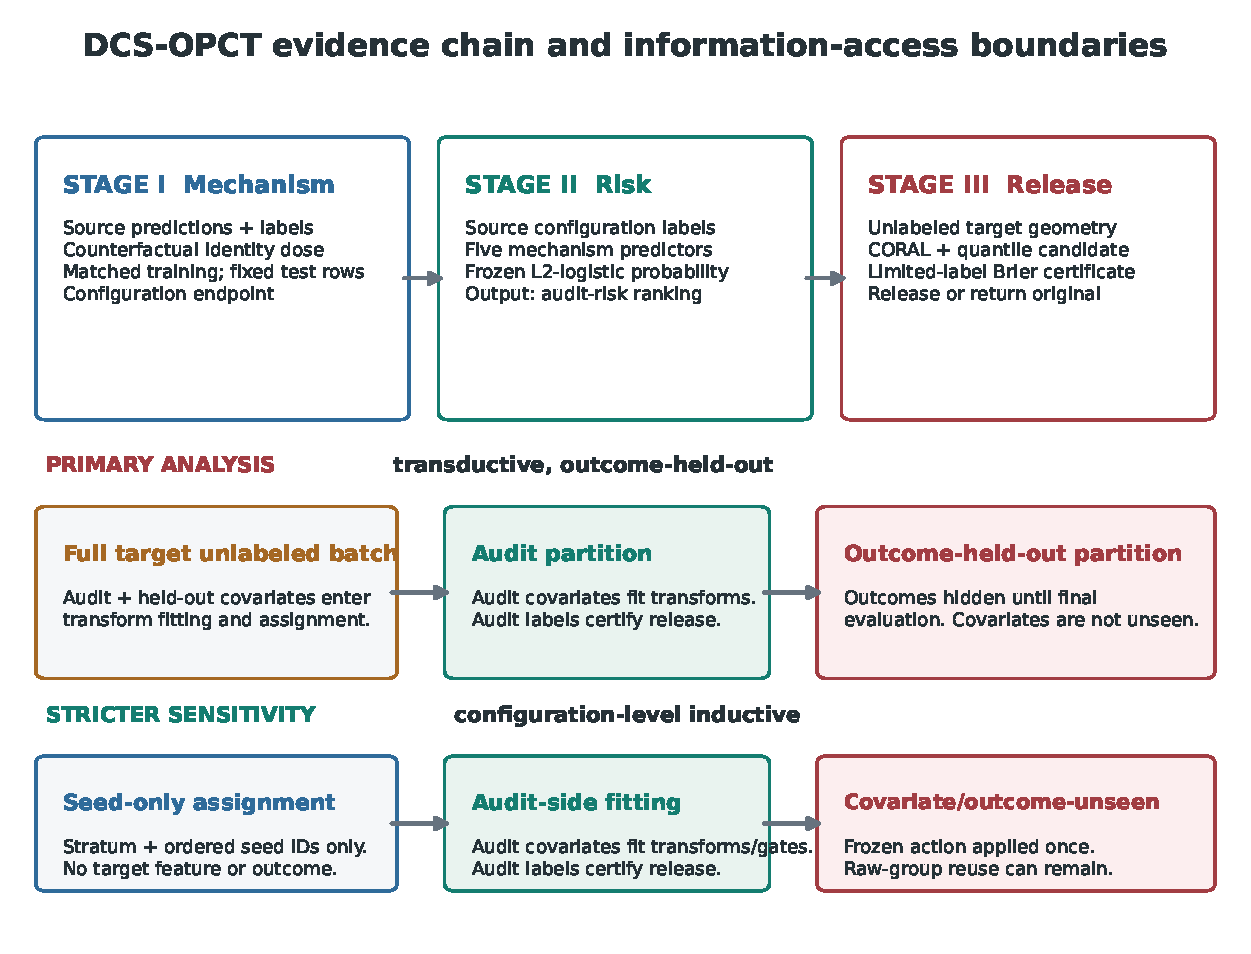
\includegraphics[width=\textwidth]{figures/fig_v11_three_stage_framework.pdf}
\caption{Three-stage DCS-OPCT evidence chain and information-access boundaries. The primary analysis is transductive because the complete unlabeled target batch may enter transformation fitting and geometry-based assignment, although final outcomes remain held out. The stricter sensitivity uses seed-only configuration assignment and audit-side fitting before one-time evaluation on covariate- and outcome-unseen configurations. A further sensitivity reconstructs endpoints from disjoint raw test groups. The final EPPVR sensitivity begins with two disjoint participant populations and independently rebuilds every target-domain emotion model before audit-only action fitting. DCS-OPCT changes audit-risk probabilities only; it never changes trial-level emotion predictions or classifier parameters.}
\label{fig:framework}
\end{figure*}

\section{Materials and methods}
\label{sec:methods}

\subsection{Study endpoint and evidence roles}

The unit transported across domains was an audit-risk probability for an experimental configuration, not an emotion prediction for an individual trial. A configuration indexed dataset, affective task, identity axis, physiological representation, classifier, split seed, and identity-opportunity dose. The binary endpoint indicated whether controlled identity opportunity produced a material increase in apparent balanced accuracy.

DEAP and MAHNOB-HCI supplied the crossed public-data mechanism experiment and trained the frozen risk model \cite{koelstra2012deap,soleymani2012mahnob}. EPPVR provided the originally locked subject-axis external test of that risk model; its failure of absolute calibration motivated probability transport. EPPVR, CASE, CEAP-360VR, SEED-IV, and DREAMER were subsequently used as retrospective development domains for DCS-OPCT \cite{sharma2019case,xue2023ceap,zheng2019emotionmeter,katsigiannis2018dreamer}. AVDOS-VR was reserved for one-shot confirmation, but the registered branch stopped before model training because its participant and feature structure violated the locked implementation contract \cite{gnacek2024avdos}. A later PPG-only analysis is reported solely as post-access exploratory robustness evidence.

FACED supplied a second external stress test with a separately preserved protocol history \cite{chen2023faced}. The registered branch required a common 32-channel EEG montage in at least 100 participants. Inspection identified 61 recordings using legacy temporal and auricular labels (T3/T4, T5/T6, and A1/A2) and 62 using revised temporal labels plus horizontal EOG channels (T7/T8, P7/P8, and HEOR/HEOL). Because auricular references and horizontal EOG are not physiologically interchangeable, no eligible 32-channel cohort existed and the registered branch was terminated before model fitting. A post-access amendment restricted the analysis to the 30 comparable EEG channels shared by all 123 participants. This common-montage analysis is exploratory only. Together, the AVDOS and FACED chronology prevents either post-access result from being presented as external confirmation.

EEGEmotions-27 was evaluated under a separate evidence role \cite{huytung2025eegemotions}. Repository-structure metadata, including participant-by-emotion availability encoded in filenames, had been inspected before registration, but no EEG sample, participant demographic row, derived feature, prediction, endpoint event, or model outcome had been accessed. The analysis was then locked before signal and outcome access at repository commit \texttt{0dfec14d177ed73c37a95f06d942e9b58e2bbf77}. It is therefore termed a separate pre-signal external robustness test rather than a pristine prospective confirmation, and it is not a member of the AMIGOS/Emognition prospective family.

The registered EEGEmotions-27 task used fixed stimulus-category polarity: emotion-video IDs 4, 20, 22, and 25 were positive, whereas IDs 5, 6, 13, 17, 18, and 24 were negative. These labels describe the assigned stimulus category and are not participant-experienced valence or arousal. One feature row represented one participant--physical-video pair after within-trial aggregation. The fixed grid used the 14-channel Emotiv X montage, three representations, two classifiers, five split seeds, five subject folds, four physical-stimulus folds, and five identity doses. Both participant and physical-video identities were held out in the dual-unseen endpoint. All GPU MLP fits used the frozen 40-epoch CUDA implementation, and the action and distribution-covered audit assignment were hashed before category-polarity outcomes entered the release decision.

EKM-ED was added as an openly accessible, prospectively reserved wearable-EEG attempt after its public metadata but before archive-member or participant-value access \cite{garciamoreno2023ekmed}. The official 4.35-GB archive was checksum verified. Its ZIP central directory and exactly two CSV header lines were recorded before a schema-specific adapter was implemented and synthetically tested. The complete adapter, tests, shared v11 dependencies, frozen risk artifacts, five seeds, five doses, 40-epoch CUDA MLP, and acceptance gates were then bound by an implementation lock. The registered tasks were participant-experienced SAM valence and arousal (1--4 low, 6--9 high, midpoint 5 excluded) for anger, sadness, happiness, and fear. Each participant--film trial required all four Muse S channels (TP9, AF7, AF8, and TP10) and three complete finite 4-s windows centered on the public film-specific key moments. A participant required at least three retained trials and both endpoint classes; at least 30 participants were required before dose construction or model fitting.

The dataset-specific emotion endpoints were not treated as one interchangeable psychological construct. DEAP, MAHNOB-HCI, EPPVR, CASE, CEAP, DREAMER, and EKM-ED used participant-rated dimensional affect under dataset-specific cut points; SEED-IV, AVDOS-VR, FACED, EEGEmotions-27, and the reserved AMIGOS protocol used fixed stimulus or segment-category contrasts. Emognition reserves participant SAM ratings but excludes the midpoint. These labels define each counterfactual experiment locally. The quantity transferred by DCS-OPCT is instead the common configuration-level event $Y_{c,d}$, conditional on that local task definition. No trial-level emotion labels, scores, or classifier outputs were pooled across datasets; the complete endpoint ontology and exclusions are reported in Supplementary Table~S1.

\subsection{Stage I: counterfactual identity dose}
\label{subsec:dose}

The crossed DEAP and MAHNOB-HCI experiment used arousal and valence, subject and stimulus identity axes, three frontal representations (all 72 features, relative power, and normalized asymmetry), two classifiers, five split seeds, and five crossed folds. The nonlinear classifier was a 40-epoch multilayer perceptron trained on CUDA; the comparison model was class-balanced logistic regression. Every test cell remained fixed across dose conditions.

For each identity axis, a class-matched control sub-block was removed from the joint-unseen training set and replaced by an identity-complete real-row exposure block of equal size. Candidate blocks preserved training size, binary class counts, test rows, and coverage of the test identities. Nominal doses were $d\in\{0,0.25,0.50,0.75,1\}$. The achieved dose was the normalized mutual information between identity and label in the exposure block, scaled within the candidate range for that test cell. This design changes identity--label opportunity without synthesizing physiology.

The estimand is a finite-sample evaluation-protocol contrast within a fixed test cell. It compares two matched training constructions that differ only in the prespecified identity-complete replacement, conditional on the available rows and the achieved opportunity level. Identification therefore requires the recorded matching invariants and deterministic construction to hold. It does not identify an unconditional causal effect of participant identity in natural deployment, and it is not a physiological intervention.

Let $c$ denote a configuration excluding dose. The exposure effect was
\begin{equation}
E_{c,d}=\operatorname{BAcc}^{\mathrm{exposed}}_{c,d}-\operatorname{BAcc}^{\mathrm{control}}_{c},
\end{equation}
where
\begin{equation}
\operatorname{BAcc}=\frac{1}{2}\left[\Pr(\hat Y=1\mid Y=1)+\Pr(\hat Y=0\mid Y=0)\right].
\end{equation}
The dose-induced amplification and material optimism event were
\begin{equation}
A_{c,d}=E_{c,d}-E_{c,0},\qquad Y_{c,d}=\mathbb{1}(A_{c,d}\geq0.02),
\end{equation}
for the four nonzero doses. The 0.02 threshold was frozen before external risk-model evaluation.
A post-hoc robustness analysis subsequently relabeled the same development configurations at thresholds from 0.01 to 0.03 and repeated leave-dataset-out validation without modifying the frozen v11 endpoint, predictors, coefficients, or external decisions. This analysis was descriptive rather than a threshold-selection procedure. We separately propagated endpoint measurement error by resampling test observations with crossed participant and physical-stimulus multinomial weights, paired across the dose and dose-zero conditions. Five thousand bootstrap draws estimated $\Pr(A_{c,d}\geq0.02)$ for every source configuration. These probabilities were used as soft labels in a post-hoc leave-dataset-out logistic sensitivity and in a soft-label evaluation of the inductive target actions. The EPPVR target analysis used participant-only resampling because no verified shared physical-stimulus identifier was available. These analyses quantify test-sample uncertainty but do not cover repeated model fitting or shared training-data uncertainty and do not replace the frozen binary endpoint.
To anchor the endpoint to an engineering consequence, we also measured absolute balanced-accuracy margins among the four candidate models under joint-unseen evaluation. For each dataset--task--seed unit, we recorded the top-two margin and all six pairwise margins. The audit-yield analysis treated the four nonzero doses for each dataset--task--representation--model--split-seed combination as one indivisible cluster. Clusters were ranked within each held-out source dataset by the maximum frozen leave-dataset-out risk probability and selected at 10\%--50\% budgets. A stratified hypergeometric test compared captured event-bearing clusters with same-budget random allocation; 10,000 random allocations characterized secondary yield metrics. ICC(1,1), design effects, effective row counts, and naive versus complete-cluster bootstrap intervals quantified within-configuration dependence. The designated post-hoc reporting cell and the full sensitivity grid are confined to the Supplementary Material. This analysis did not alter the risk model, v11 actions, or release thresholds.

\subsection{Model-selection consequences}
\label{subsec:ranking}

The practical effect of identity exposure was evaluated by comparing the ordering of candidate representation--model pairs under an exposed protocol with their ordering under joint-unseen testing. For each dataset, task, exposure condition, and split seed, the analysis recorded whether the nominal winner changed, whether the change was material, Kendall's rank correlation, and the fraction of inverted model pairs. Deployment regret was
\begin{equation}
R=\operatorname{BAcc}^{\mathrm{joint}}(m^*_{\mathrm{joint}})-\operatorname{BAcc}^{\mathrm{joint}}(m^*_{\mathrm{exposed}}),
\end{equation}
where $m^*_{\mathrm{exposed}}$ is selected under identity exposure and $m^*_{\mathrm{joint}}$ is the oracle winner under joint-unseen evaluation. Material reversal required both a different winner and a practically relevant joint-unseen performance loss.

\subsection{Stage II: frozen identity-shortcut audit-risk model}
\label{subsec:riskmodel}

Only subject-axis counterfactual rows from DEAP and MAHNOB-HCI were used to train the primary risk model. Dose-zero rows served only as anchors, leaving 480 nonzero-dose configurations. These rows arose from only two independent source datasets; configuration-level sample size must therefore not be interpreted as domain-level replication ($n_{domain}=2$). The model was L2-regularized logistic regression with $C=0.1$:
\begin{equation}
p_{c,d}=\sigma\left(\beta_0+\boldsymbol{\beta}^{\top}\mathbf{x}_{c,d}\right).
\end{equation}
The predictor vector contained five prespecified mechanism variables: change in achieved label opportunity from dose zero, metadata-prior opportunity, identity-probe encoding margin above chance, the opportunity-change by encoding-margin interaction, and an ordinal model-capacity indicator. Dataset identity, dataset size, task identity, representation identity, model identity, and all equivalent proxies were excluded from the primary model.

Leave-dataset-out predictions determined admissibility. Within each training fold, the operating threshold was selected from training-only out-of-fold predictions to maximize balanced accuracy. The final frozen threshold was 0.18619. A public-data development gate required AUROC at least 0.65, average precision divided by event prevalence at least 1.5, positive Brier skill, balanced accuracy at least 0.60 at the training-only threshold, and positive mechanism-direction coefficients in both dataset-transfer fits. The fitted model and all predictor tables were checksum locked before the EPPVR target was evaluated.

\subsection{Why probability transport was required}

The EPPVR test distinguished ranking transport from probability transport. AUROC and precision-recall enrichment quantify whether high-risk configurations tend to be ranked earlier, whereas probability calibration determines whether a value such as 0.30 can be interpreted as approximately 30\% event risk. The latter is required for thresholded audit allocation and benefit--risk decisions. Calibration was measured by the Brier score \cite{brier1950verification}:
\begin{equation}
\operatorname{BS}(p)=\frac{1}{n}\sum_{i=1}^{n}(p_i-y_i)^2.
\end{equation}
For an adapted probability $p^{(A)}$ and the frozen identity probability $p^{(I)}$, positive Brier gain was
\begin{equation}
G_{\mathrm{BS}}=\operatorname{BS}(p^{(I)})-\operatorname{BS}(p^{(A)}).
\end{equation}

\subsection{Stage III: DCS-OPCT probability action}
\label{subsec:dcs}

DCS-OPCT operates on the mechanism-feature table of the frozen audit-risk model. Two separately constructed label-free feature transforms map target configurations toward the source-domain geometry. The primary component uses CORAL to align the target covariance to the source covariance \cite{sun2016coral}. The complementary witness uses marginal quantile mapping. Both use the same target configuration batch and frozen risk model, so their agreement is an applicability diagnostic rather than statistically independent confirmation. Each transformed feature table is passed through the unchanged frozen risk model, producing two base probability vectors.

The base probabilities are projected onto a positive-slope order-preserving calibration map
\begin{equation}
T_{a,b}(p)=\sigma\left[a\operatorname{logit}(p)+b\right],\qquad a>0.
\end{equation}
For component $k$, identity-probability logits were the inputs and the label-free CORAL or quantile base probabilities $\widetilde p_i^{(k)}$ were soft targets. The fitted parameters minimized
\begin{equation}
\mathcal{L}_k(a,b)=\frac{1}{n}\sum_{i=1}^{n}\left[T_{a,b}(p_i^{(I)})-\widetilde p_i^{(k)}\right]^2+\lambda\left[(a-1)^2+b^2\right],
\end{equation}
subject to $0.1\leq a\leq5$ and $|b|\leq5$. No target outcome entered this optimization. Parameters were fitted on CUDA for 500 epochs with learning rate 0.03 and regularization $\lambda=10^{-4}$. The scale was constrained to $[0.1,5]$ and the logit shift to $[-5,5]$. Each component was ineligible when its absolute mean probability displacement exceeded 0.10, Spearman rank was below 0.999999, or any order inversion occurred. Because $a>0$, an eligible OPCT map is strictly increasing and preserves all rankings and ties.

Let $\Delta^{(P)}=p^{(P)}-p^{(I)}$ and $\Delta^{(W)}=p^{(W)}-p^{(I)}$ be the primary and witness displacements. Agreement was quantified as
\begin{align}
G_{\mathrm{dir}}&=\frac{1}{|I|}\sum_{i\in I}\mathbb{1}\left(\Delta_i^{(P)}\Delta_i^{(W)}\geq0\right),\\
G_{\cos}&=\frac{\langle\Delta^{(P)},\Delta^{(W)}\rangle}{\|\Delta^{(P)}\|_2\|\Delta^{(W)}\|_2},\\
G_{\mathrm{dis}}&=\frac{1}{n}\sum_i\frac{|\Delta_i^{(P)}-\Delta_i^{(W)}|}{|\Delta_i^{(P)}|+|\Delta_i^{(W)}|+\epsilon},
\end{align}
where $I$ contains configurations with non-negligible displacement by at least one component. Release required $G_{\mathrm{dir}}\geq0.90$, $G_{\cos}\geq0.90$, and $G_{\mathrm{dis}}\leq0.35$. Failure of either component or any witness criterion set the candidate action to identity before labels were accessed.

\subsection{Unlabeled audit assignment and limited-label certification}
\label{subsec:audit}

Eligible actions still required target-domain certification. Configurations were grouped into complete four-dose clusters indexed by task, representation, model, and split seed. Each cluster was summarized without labels by seven geometry quantities: mean and standard deviation of identity probability, adapted probability, and probability displacement, plus the decision-flip fraction at 0.5. These features were standardized across target clusters.

Within every task-by-representation-by-model stratum, the five split-seed clusters were divided between audit and held-out partitions. A deterministic parity rule allocated three audit clusters to half the strata and two to the remainder, yielding exactly one half of all clusters. Every subset of the required size was enumerated, and the selected subset minimized
\begin{equation}
J(S)=\|\boldsymbol\mu_S-\boldsymbol\mu_G\|_2^2+0.05\|\boldsymbol\sigma_S-\boldsymbol\sigma_G\|_2^2,
\end{equation}
where $G$ denotes all clusters in the stratum. Ties were resolved lexicographically by split-seed identifier. No outcome, loss, AUROC, certificate, or held-out result entered assignment.

Brier gain was certified with 5,000 bootstrap repetitions that resampled complete four-dose clusters within task-by-representation-by-model strata while preserving each stratum's audit count. With one registered candidate, the one-sided familywise lower confidence bound had to exceed 0.001. AUROC noninferiority used a margin of $-0.02$. An analytic zero AUROC difference was accepted only after rank at least 0.999999 and zero inversions had been verified. A released action was then evaluated once on the outcome-held-out half; otherwise identity was retained. In this primary retrospective analysis, however, the complete unlabeled target configuration table contributed to transformation fitting and distribution-covered assignment. The primary estimand is therefore transductive performance conditional on the observed target batch, not performance for a covariate-unseen future batch.

We added a stricter configuration-level inductive sensitivity. Within each task--representation--model stratum, audit clusters were assigned by a deterministic rule using only the ordered split-seed identifiers and stratum labels; no target feature or outcome entered assignment. Source statistics and audit-side unlabeled target features alone estimated the CORAL matrix, empirical quantile maps, and positive-slope OPCT parameters. Applicability and witness gates and the labeled certificate were then evaluated on the audit side, after which the frozen map was applied once to held-out configurations whose covariates and outcomes had not been accessed. This sensitivity removes held-out-covariate access but does not remove reuse of underlying participant or stimulus observations across split-seed configurations.

We therefore added a second, nested raw-group sensitivity. Participant identifiers were deterministically divided into disjoint audit and evaluation sets. For CASE, CEAP, SEED-IV, and DREAMER, verified physical-stimulus identifiers were also divided, and endpoint labels were independently reconstructed on the audit-participant--audit-stimulus and evaluation-participant--evaluation-stimulus diagonals. EPPVR used participant-disjoint rows only because no cross-participant physical-stimulus identifier was verified. Configuration assignment and transform fitting followed the inductive protocol; the release certificate used only audit-group endpoint labels, and final Brier gain used only evaluation-group endpoint labels. This design removes shared raw test participants and identified stimuli but still reuses trained emotion models and can share their training rows across split seeds.

Finally, we performed a raw-partition-first EPPVR sensitivity. Sorted participant identifiers were assigned by parity, without reading covariates or outcomes, to two disjoint 15-participant populations. Inside each population we independently reconstructed all identity-dose blocks, trained all linear and 40-epoch CUDA MLP emotion models, generated test predictions, fitted identity probes, and assembled the 320 nonzero-dose configuration endpoints. Across the two populations this required 9,600 emotion-model fits and 160 identity-probe fits. No participant, global raw row, training row, or fitted target-domain emotion model crossed the population boundary. CORAL, quantile maps, positive-slope OPCT parameters, component and witness gates, distribution-covered audit assignment, and the 160-configuration certificate were estimated from the audit population only. The resulting release-or-return-original decision was then applied once to all 320 evaluation-population configurations. This is a single retrospective EPPVR population split, not a new-dataset, cross-session, stimulus-independent, or prospective external validation.

\subsection{Matched audit-budget decision analysis}
\label{subsec:budget}

The fixed v11 held-out half was retained as the common evaluation set. Within the already assigned audit half, 100 seeded balanced cluster orderings of the same fixed data generated nested 20\%, 40\%, 60\%, 80\%, and 100\% label budgets. These corresponded to 32--160 labeled configurations for EPPVR, CASE, and CEAP and 24--120 for SEED-IV and DREAMER. No held-out outcome entered fitting, certification, or budget selection. The 100 orderings were conditional allocation-sensitivity replicates, not independent dataset or participant replications.

Ten actions were compared. Selective DCS-OPCT used its label-free candidate and spent the available labels only on the stratified release certificate. Unconditional DCS-OPCT applied the same candidate without certification as a diagnostic. Positive-slope target Platt scaling, target isotonic regression, monotone beta calibration, and temperature scaling were fitted directly on all labels available at each budget. The beta map was
\begin{equation}
q_{\beta}(p)=\sigma\!\left[a\log p-b\log(1-p)+c\right],\qquad a,b>0,
\end{equation}
which is more flexible than Platt scaling while preserving probability rank \citep{kull2017beta}. Temperature scaling used $q_T(p)=\sigma[s\operatorname{logit}(p)]$, $s>0$, as a restricted no-intercept control \citep{guo2017calibration}. Split-fit/certified Platt and beta comparators divided the ordered clusters alternately into fitting and certification subsets; a fitted map was released only when the independent subset passed the same Brier lower-bound threshold. To use the complete audit budget without in-sample certification, same-audit cross-fit comparators reversed the two folds, combined both out-of-fold prediction sets for certification, and, only after a positive certificate, refitted the released map on all audit labels for held-out evaluation. Thus, cross-fit certification used every audit label while ensuring that each probability entering the certificate was produced by a map fitted on the opposite fold. All parametric calibrators were optimized on CUDA for 1,000 epochs.

A separate nearest-neighbor comparison used the stricter inductive assignment and its full audit-label budget. The CPCS-style adaptation trained a balanced logistic domain discriminator on standardized source configurations and audit-side unlabeled target configurations. For source configuration $i$, the estimated covariate-shift weight was
\begin{equation}
w_i=\frac{\widehat P(D=T\mid\mathbf{x}_i)}{1-\widehat P(D=T\mid\mathbf{x}_i)}\frac{n_S}{n_T},
\end{equation}
clipped to $[0.05,20]$ before mean normalization. A positive-slope weighted Platt map was fitted to the source endpoint labels only; no target label entered candidate fitting. The candidate then faced the same target audit certificate as DCS-OPCT. This is a configuration-level CPCS-style adaptation, not a verbatim instance-classifier reproduction. TransCal was not instantiated because its primary formulation calibrates logits from a target-adapted task classifier, whereas the present object is an unchanged audit-risk model with no target-adapted classifier. For an empirical non-interventional reference, an ATC-style confidence threshold was selected so that source threshold exceedance matched source hard-classification accuracy; target accuracy was then estimated from the unlabeled held-out confidence distribution. Because ATC outputs one aggregate accuracy estimate rather than corrected configuration probabilities, Brier gain, probability AUROC change, and release harm are not defined for that row.

For method $m$, material negative transfer in repetition $r$ was
\begin{equation}
N_{m,r}=\mathbb{1}\!\left(A_{m,r}=1\ \land\ G_{\mathrm{BS},m,r}<-0.001\right),
\end{equation}
where $A_{m,r}$ indicates that a non-identity action was released. We reported release rate, mean held-out Brier gain, material-negative-transfer frequency, and AUROC noninferiority failure frequency. The plotted 95\% intervals combine a random audit-order draw with stratified complete-cluster resampling of the fixed held-out half. Formal DCS-versus-comparator inference used 20,000 paired bootstrap repetitions for the null of zero mean paired Brier-gain difference, 100,000 paired sign-randomization repetitions for exchangeability of the paired gain signs, and exact McNemar tests for equal discordant material-negative-event probabilities. $P$ values were Holm-adjusted across all 150 dataset-by-budget-by-comparator cells. One-sided 95\% Clopper--Pearson upper bounds were also reported for observed material-negative frequency among released actions. These analyses quantify retrospective design sensitivity on reused held-out halves, not prospective external-validation uncertainty or future-domain risk.

Three simplified end-to-end variants were reconstructed from the same frozen actions, assignments, and 720-configuration action-stage budget ceiling. Certificate only removed both unlabeled gates, single unlabeled gate retained only the primary component screen, and full DCS-OPCT retained the component screen and complementary witness. This same-assignment diagnostic counted labels entering action selection; it did not refit candidates, change thresholds, or estimate prospective sample complexity. We also performed a post-hoc local action-stability analysis over eight frozen decision parameters. Each parameter was perturbed one at a time over two more permissive and two stricter settings, followed by a three-level joint cube over all eight parameters. These perturbations diagnose local brittleness of archived decisions and were not used for threshold selection. The provenance and inferential role of every endpoint, applicability, and release threshold are summarized in Supplementary Table~S8; post-hoc stability analyses were never used to select or retune these values.

\subsection{Computational and reproducibility controls}

All neural fits and OPCT optimization used an NVIDIA GeForce RTX 4070 Ti SUPER. Five deterministic split seeds were used throughout: 20260813, 20260829, 20260911, 20260923, and 20261007. Progress reporting covered preflight construction, model fitting, transformation fitting, and bootstrap stages. The raw-partition-first analysis additionally stored a 9,760-row fit-provenance ledger containing population membership, train/test participant sets, global-row-set hashes, and overlap checks for every emotion-model and identity-probe fit. Output manifests record input paths, settings, GPU device, code checksums, and frozen-model checksums. Independent validators reproduce the development, comparator, external-boundary, sensitivity, and submission-artifact checks. A single release-readiness driver compiles the analysis code, runs static checks, refreshes the prospective pre-access CUDA stacks, verifies their code hashes and the frozen manifest, and reruns the submission validator. Failed method versions, execution defects, and external-protocol incompatibilities were retained rather than overwritten; exact validator inventories are reported in the Supplementary Material.

The current immutable reproducibility inventory contains 214 files and passed 23/23 checks. The release-readiness driver passed 6/6 gates, including the fail-closed external-arrival detector, whose own validation passed 7/7. AMIGOS and Emognition remained blocked by external data access. EKM-ED progressed beyond readiness to a checksum-verified, implementation-locked prospective attempt, but failed the frozen structural endpoint before model fitting. Neither software readiness nor structural failure constitutes external effectiveness or future-domain non-harm evidence.

\section{Results}
\label{sec:results}

\subsection{Counterfactual dose separates opportunity, encoding, and utilization}

The complete crossed experiment contained DEAP and MAHNOB-HCI, two affective tasks, two identity axes, three representations, two model families, five split seeds, and five dose levels. Opportunity was successfully varied within the candidate range while preserving every construction invariant. The response was heterogeneous rather than universally monotonic: increasing identity--label mutual information sometimes amplified exposure effects, but the direction and magnitude depended on dataset, task, representation, and model. Figure~\ref{fig:dose-ranking}A shows this separation most clearly: mean subject-axis amplification increased with dose in both datasets, whereas stimulus-axis means remained near zero over most of the range. The subject-axis prevalence of the prespecified material event also varied by dataset and dose (Fig.~\ref{fig:dose-ranking}B). These results reject the shortcut assumption that high identity decodability alone determines use by the emotion classifier and motivate a probabilistic risk endpoint rather than a universal deterministic rule.

\subsection{Identity exposure altered model selection}

Exposure-biased rankings frequently differed from joint-unseen rankings. For DEAP arousal under subject exposure, the nominal winner changed in 80\% of split seeds, the material winner-reversal rate was 60\%, and mean joint-unseen regret was 0.0212 balanced accuracy. DEAP valence showed a 40\% material subject-exposure reversal and mean regret of 0.0205. MAHNOB-HCI arousal showed a 60\% material subject-exposure reversal and mean regret of 0.0229. Pairwise inversion fractions were 0.733, 0.753, and 0.480 in these three settings, respectively. Stimulus exposure generally produced smaller regret, although heterogeneous reversals remained. Figure~\ref{fig:dose-ranking}C places the material reversal rates beside the corresponding deployment regrets. Identity exposure therefore affected not only reported performance but also which system would be chosen for deployment.

\begin{figure*}[t]
\centering
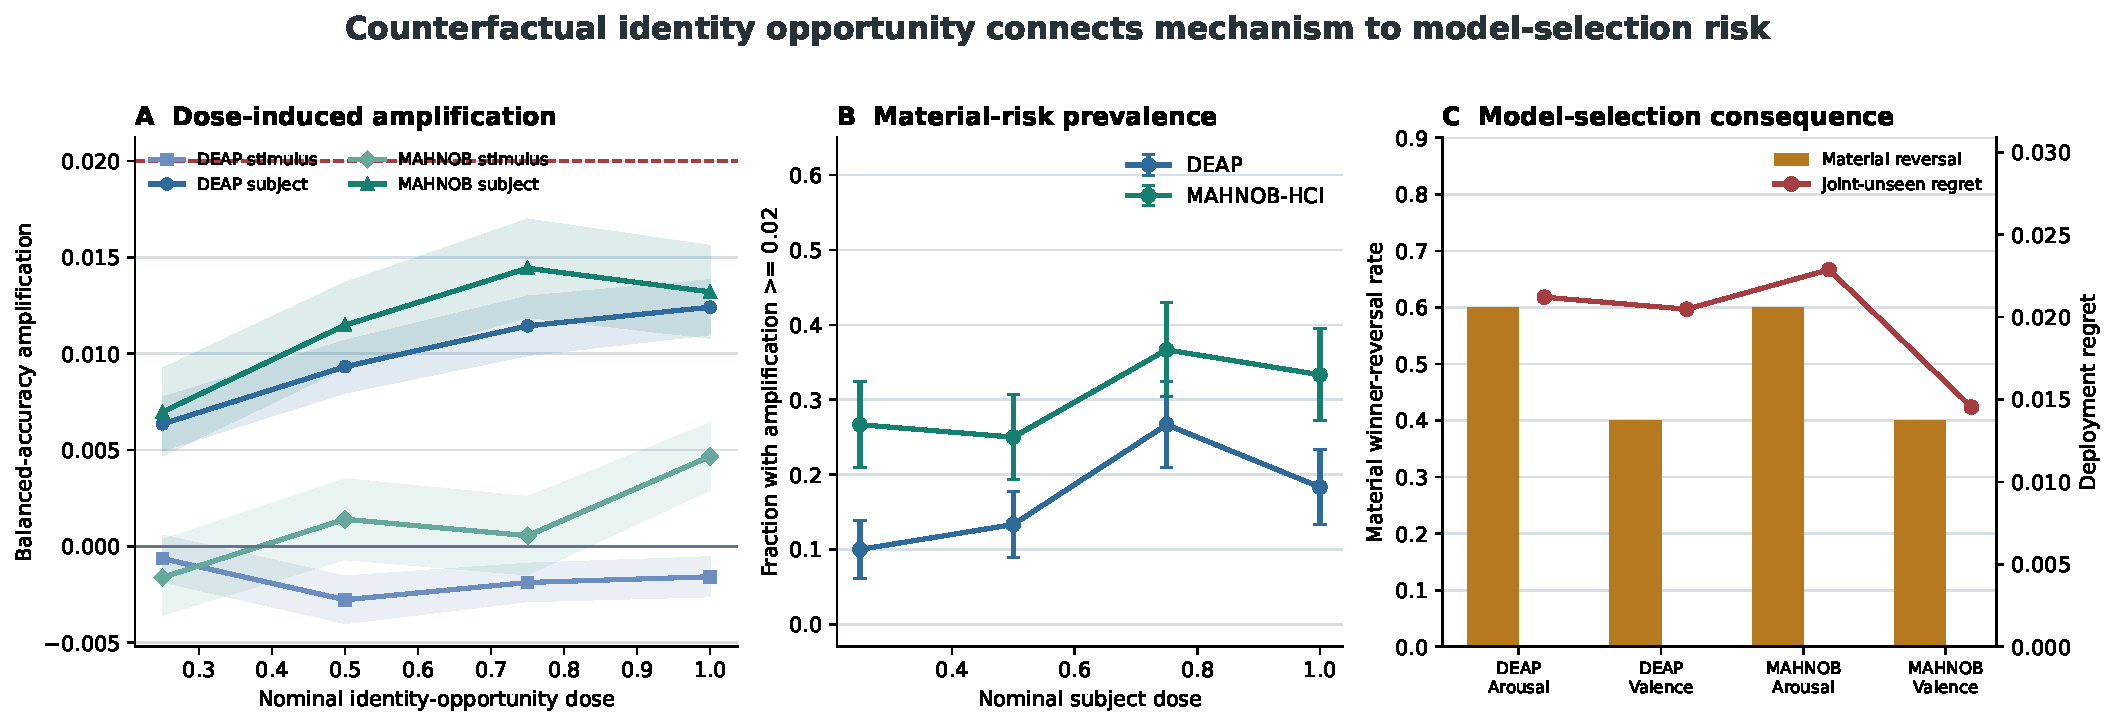
\includegraphics[width=\textwidth]{figures/fig_v11_dose_and_ranking_consequences.pdf}
\caption{Mechanism and model-selection consequences of controlled identity opportunity. (A) Mean dose-induced balanced-accuracy amplification, with shaded uncertainty bands, for subject and stimulus identity axes; the dashed line marks the prespecified 0.02 materiality threshold. (B) Fraction of subject-axis configurations meeting the material event definition at each nonzero dose; error bars summarize variation across crossed task, representation, model, and split-seed cells. (C) Material winner-reversal rate and mean joint-unseen deployment regret under subject exposure. The panels describe heterogeneous evaluation effects and selection consequences, not physiological dose--response relationships.}
\label{fig:dose-ranking}
\end{figure*}

\subsection{The frozen risk model transferred ranking but not EPPVR calibration}

Across the two public leave-dataset-out tests, the frozen risk model met every development requirement. When DEAP was held out, AUROC was 0.698, average-precision lift was 2.414, Brier skill was 0.100, and training-threshold balanced accuracy was 0.607. When MAHNOB-HCI was held out, the corresponding values were 0.735, 1.693, 0.123, and 0.619. The minimum values across the two transfers therefore passed the frozen gate.

In the post-hoc endpoint analysis, thresholds 0.01 and 0.015 failed at least one descriptive transfer floor. Thresholds 0.02 and 0.025 met all four floors and retained at least 20 events in each held-out dataset. Although 0.03 also met the metric floors, DEAP contained only eight events. The frozen 0.02 endpoint therefore lies at the lower edge of the empirically stable tested region rather than at an isolated favorable value; this finding does not confer physiological meaning or establish threshold optimality (Supplementary Material).

The crossed test-sample bootstrap exposed a stricter limitation. Of 240 source configurations per dataset, the 95\% amplification interval crossed 0.02 in 238 DEAP and all 240 MAHNOB-HCI configurations, and no configuration had a lower bound at or above 0.02. Replacing hard events with bootstrap event probabilities improved soft-label Brier score relative to the frozen hard-label model from 0.0435 to 0.0350 when DEAP was held out and from 0.0608 to 0.0572 when MAHNOB-HCI was held out, but hard-label AUROC decreased and several coefficient signs differed between transfers. The mechanism coefficients therefore are not interpreted as measurement-error-stable effects. At the action stage, the inductive EPPVR and CASE corrections retained positive soft-label Brier gains of 0.0161 and 0.0209, respectively; all three abstained domains remained unchanged. This sensitivity preserves the direction of the two released actions while showing that binary event counts and coefficient-level interpretation are fragile.

The engineering-anchor analysis gave the 0.02 magnitude a concrete operational interpretation. Seventeen of 20 joint-unseen model-selection units (85\%, cluster-bootstrap 95\% CI 70--100\%) had a top-two candidate margin no greater than 0.02, and 65 of 120 model pairs (54.2\%, 44.2--65.0\%) were separated by no more than this amount. In the corrected complete-cluster analysis, a 20\% budget selected 24 clusters, corresponding to 96 configuration labels, and captured 19 of 56 event-bearing clusters (33.9\%) versus a random mean of 20.0\% (stratified exact $p=0.000345$). The same allocation captured 43 of 114 event configurations (37.7\%) and 37.4\% of amplification exceeding the material threshold. Maximum, mean, and median aggregation of the four frozen risk scores selected the same 24 clusters and produced identical yield. Dependence was substantial: material-event ICC was 0.420 and reduced the design-effect-based effective row count from 480 to approximately 212; complete-cluster intervals were 1.30--1.75 times as wide as naive row-bootstrap intervals across the reported endpoints and datasets. We therefore added a more conservative post-hoc sensitivity that treated each dataset--task--split-seed family as one indivisible unit. This produced 20 conditional higher-level blocks, each containing all representations, models, and nonzero doses. At the 20\% budget, two whole blocks per source dataset were selected. All 2,025 valid same-budget allocations were enumerated exactly, and uncertainty for event prevalence and mean amplification was estimated by stratified resampling of these blocks. At the higher dataset--task--seed level, the same 20\% label budget selected four blocks and captured 26.3\% of event rows and 25.9\% of material excess, corresponding to 1.316-fold event enrichment. However, neither quantity exceeded the exact whole-block random-allocation distribution ($p=0.207$ and $p=0.260$, respectively). Maximum, mean, and median block-risk aggregation again selected the same blocks. Thus, the significant complete-configuration result does not persist as statistically persuasive workflow-level yield under the coarser dependence unit. The combined evidence supports configuration prioritization within the fixed development sources, not a general audit-allocation benefit across tasks, seeds, or future domains (Supplementary Material).

The locked EPPVR test exposed a different pattern. AUROC was 0.666 (95\% CI 0.558--0.767) and average-precision lift was 2.192 (1.510--3.250), satisfying the discrimination and enrichment criteria. Brier skill was $-0.128$ ($-0.325$--0.032), however, and balanced accuracy at the frozen threshold was 0.599 (0.520--0.675), narrowly below the required 0.60. Mean predicted risk was 0.294 compared with event prevalence 0.163, and the observed-to-expected ratio was 0.553. Thus, audit priority transferred more successfully than absolute probability or the operating point. This failure was retained and became the direct design target for DCS-OPCT.

We also tested whether source breadth alone removed this instability. In a post-hoc seven-dataset analysis, 1,920 subject-axis configurations from DEAP, MAHNOB-HCI, EPPVR, CASE, CEAP, SEED-IV, and DREAMER were evaluated by nested leave-one-dataset-out validation. The five frozen mechanism predictors were retained, and pooled, equal-domain, and smooth worst-domain L2 logistic models were fitted on CUDA. For the equal-domain model, all 35 outer-fold mechanism coefficients were positive and weighted Brier score improved by 0.0111 relative to the frozen two-source probabilities. Nevertheless, median held-out AUROC was only 0.616, four of seven domains reached AUROC 0.60, and median nested-threshold balanced accuracy was 0.592. The prespecified retrospective robustness gate therefore failed. Broader pooling improved average probability error but did not establish transferable discrimination or operating points (Supplementary Figure~S5 and Table~S12).

\subsection{DCS-OPCT released correction in three development domains}

Figure~\ref{fig:actions} summarizes the six domain-level decisions. EPPVR, CASE, and CEAP passed both component and witness gates. Their directional agreement values were 0.938, 0.994, and 0.925; displacement cosines were 0.997, 1.000, and 0.947; and normalized disagreements were 0.209, 0.080, and 0.208. Every adapted probability vector retained rank 1.0 and zero order inversions.

The distribution-covered audit certified all three eligible actions (Table~\ref{tab:actions}). Audit Brier gains were 0.0222 for EPPVR, 0.0253 for CASE, and 0.0102 for CEAP. Their one-sided lower confidence bounds were 0.0096, 0.0112, and 0.0019, all above the fixed 0.001 threshold. On the outcome-held-out halves, gains were 0.0263, 0.0485, and 0.0085. AUROC change was exactly zero after order preservation was verified, and no released action showed material negative transfer.

The covariate-unseen sensitivity separated results that required transductive target-batch access from those that did not. EPPVR and CASE again passed the component, witness, and certificate gates; their audit lower bounds were 0.0152 and 0.0212 and held-out Brier gains were 0.0226 and 0.0406. SEED-IV and DREAMER remained identity actions. CEAP passed the component screen but failed the audit-side quantile witness and therefore reverted to identity before outcome evaluation. No inductively released action showed material negative transfer, and all maps preserved probability order. Thus, the positive CEAP result is conditional on the original transductive construction, whereas EPPVR and CASE provide the stronger configuration-level inductive sensitivity evidence (Supplementary Material).

Raw-group separation further narrowed that evidence. EPPVR remained applicable and certified; its audit Brier-gain lower bound was 0.0254 and its participant-disjoint evaluation gain was 0.0135. CASE remained applicable but its certificate lower bound fell to $-0.0091$, so the action returned the original probability. CEAP and DREAMER failed the audit-side witness and SEED-IV failed the component screen. Thus, only EPPVR retained a released positive action after simultaneous configuration-level covariate holdout and raw test-participant separation. This remains the strongest positive independence sensitivity, but it retained shared model-training rows.

The raw-partition-first EPPVR sensitivity removed that remaining overlap. Each 15-participant population produced 320 configurations after independently rebuilding every dose experiment and fitted emotion model. Material-event prevalence was 0.2219 in the audit population and 0.2719 in the evaluation population. However, the audit-fitted CORAL and quantile OPCT components required mean probability shifts of $-0.2122$ and $-0.2030$, both beyond the frozen absolute limit of 0.10. The component screen therefore stopped the action before the certificate or evaluation outcomes could authorize a correction. All 320 evaluation configurations received the original probability, giving gain and AUROC change of zero by construction. The independent validator passed 21/21 checks, including disjoint participants, raw rows, training rows, and fitted target-domain models. Figure~\ref{fig:independence-ladder} shows that the release set contracts monotonically as information and raw-data separation become stricter. The final stop is evidence of target-batch dependence and fail-closed execution, not calibration effectiveness or proof of safety.

\begin{figure*}[t]
\centering
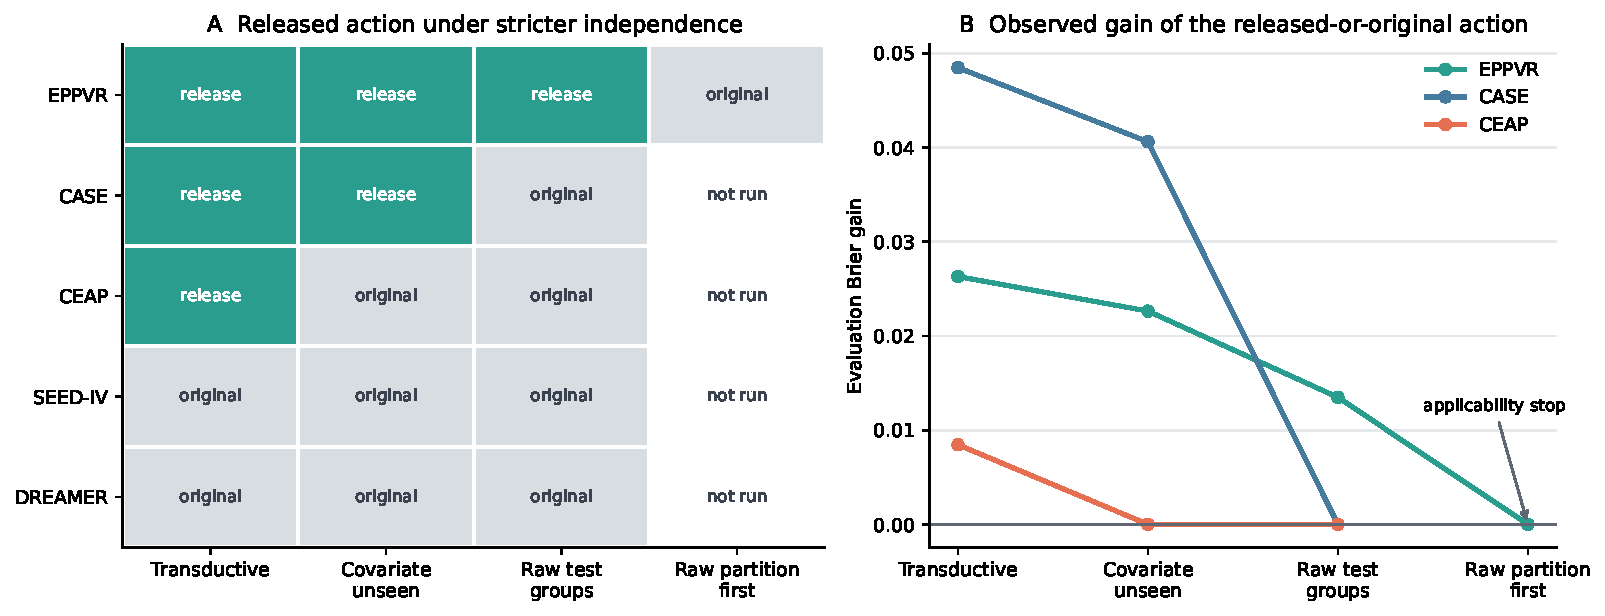
\includegraphics[width=\textwidth]{figures/fig_v11_independence_ladder.pdf}
\caption{Independence ladder for the retrospective DCS-OPCT evidence. (A) Released correction versus return-original action as target-covariate, raw-test-group, and finally complete training-population overlap are removed. White cells were not rerun under the EPPVR-only raw-partition-first protocol. (B) Evaluation Brier gain of the released-or-original action. Zero at a return-original action is non-intervention, not successful calibration. The fully participant- and training-row-disjoint EPPVR analysis stopped at the frozen unlabeled applicability gate.}
\label{fig:independence-ladder}
\end{figure*}

\begin{figure}[t]
\centering
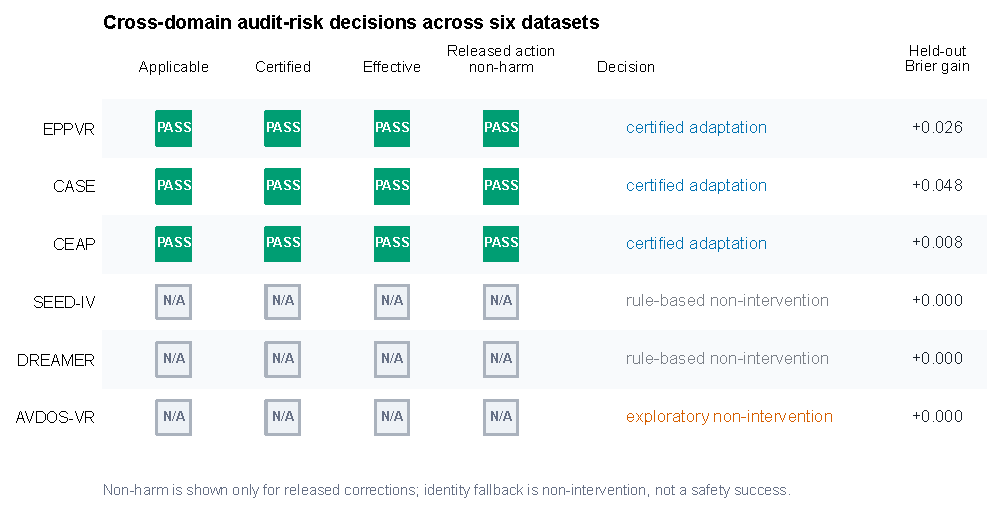
\includegraphics[width=\textwidth]{figures/fig_v11_six_dataset_action_matrix.pdf}
\caption{Domain-level DCS-OPCT decisions. Correction was released only when the unlabeled component and witness gates passed and the distribution-covered audit certified Brier improvement. Released-action non-harm is evaluated only for an applied correction; identity denotes non-intervention and is not counted as either effectiveness or a safety success. AVDOS-VR is post-access exploratory evidence.}
\label{fig:actions}
\end{figure}

\begin{table*}[t]
\centering
\caption{DCS-OPCT v11 audit-risk calibration actions and outcomes. AVDOS-VR and FACED are post-access exploratory analyses and cannot support confirmatory effectiveness.}
\label{tab:actions}
\small
\resizebox{\textwidth}{!}{%
\begin{tabular}{lllrrrrl}
\toprule
Dataset & Evidence role & Action & Audit gain & LCB & Held-out gain & $\Delta$AUROC & Outcome \\
\midrule
EPPVR & Development & CORAL + OPCT & 0.0222 & 0.0096 & 0.0263 & 0.0000 & certified adaptation \\
CASE & Development & CORAL + OPCT & 0.0253 & 0.0112 & 0.0485 & 0.0000 & certified adaptation \\
CEAP & Development & CORAL + OPCT & 0.0102 & 0.0019 & 0.0085 & 0.0000 & certified adaptation \\
SEED-IV & Development & identity & -- & -- & 0.0000 & 0.0000 & rule-based non-intervention \\
DREAMER & Development & identity & -- & -- & 0.0000 & 0.0000 & rule-based non-intervention \\
AVDOS-VR & Exploratory & identity & -- & -- & 0.0000 & 0.0000 & exploratory non-intervention \\
FACED & Exploratory & identity & -- & -- & -- & -- & inapplicable; endpoint event-free \\
\bottomrule
\end{tabular}
}
\end{table*}

Figure~\ref{fig:gains} separates audit evidence from held-out evaluation. The held-out gain exceeded the corresponding audit estimate for EPPVR and CASE and remained positive for CEAP, despite CEAP's lower-bound certificate lying close to the release threshold. These differences are important because the audit was used only for the release decision; the held-out half was not involved in action selection.

\begin{figure}[t]
\centering
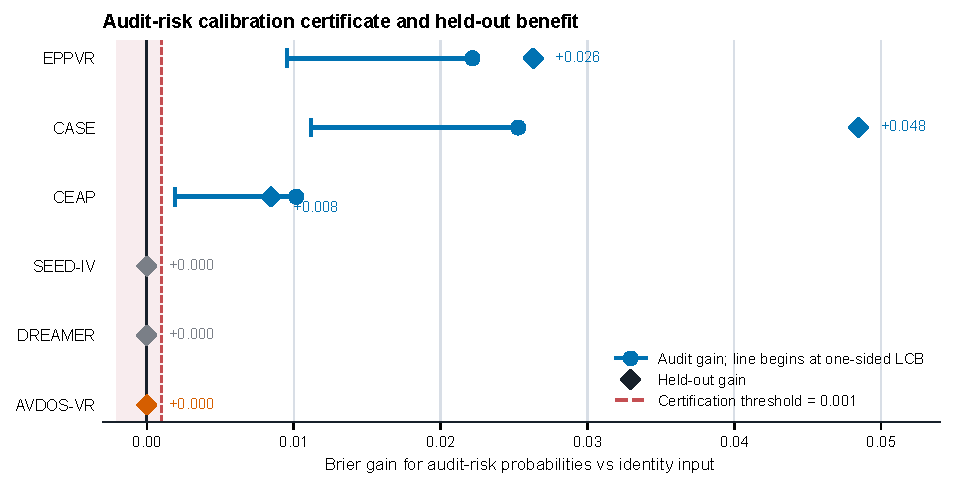
\includegraphics[width=\textwidth]{figures/fig_v11_audit_and_heldout_gain.pdf}
\caption{Brier gains for the three released development actions. Audit points show observed gain and the one-sided familywise lower confidence bound from 5,000 stratified complete-cluster bootstrap repetitions. Held-out points are evaluated on the retained half of target configurations. Positive values favor DCS-OPCT.}
\label{fig:gains}
\end{figure}

\subsection{Budget curves exposed a calibration-gain--intervention-risk tradeoff}
\label{subsec:budget-results}

The minimum-budget analysis used 32 labeled configurations in EPPVR, CASE, and CEAP and 24 in SEED-IV and DREAMER. DCS-OPCT released 83\%, 83\%, and 71\% of EPPVR, CASE, and CEAP repetitions, producing mean held-out Brier gains of 0.0218, 0.0402, and 0.0060. It abstained in every SEED-IV and DREAMER repetition because their label-free applicability gates had already failed. No DCS release produced material negative transfer at any tested budget, but the one-sided 95\% upper bounds among released actions were 2.95--4.64\% rather than zero (Fig.~\ref{fig:budget-tradeoff}).

Direct target Platt scaling achieved comparable or larger average gain in EPPVR and CASE at the minimum budget, but material negative transfer occurred in 6\% and 5\% of repetitions. The corresponding frequencies were 69\% in SEED-IV, 53\% in DREAMER, and 25\% in CEAP, where mean gains were negative. Monotone beta calibration closely reproduced this pattern: its frequencies were 6\%, 69\%, 53\%, 6\%, and 28\%, with negative mean gains in SEED-IV, DREAMER, and CEAP. Isotonic calibration was less stable, with minimum-budget material-negative frequencies of 17--99\% and AUROC noninferiority failures in four domains. Splitting the same label budget between fitting and certification reduced intervention frequency, but neither the Platt nor beta comparator eliminated material negative transfer across the five domains at the minimum budget. Same-audit two-fold cross-fitting did not close this gap. Cross-fit-certified Platt released in 40\%, 21\%, 27\%, 45\%, and 29\% of repetitions for EPPVR, SEED-IV, DREAMER, CASE, and CEAP; material-negative frequencies were 0\%, 21\%, 17\%, 0\%, and 13\%. Cross-fit beta gave the same qualitative result, with harmful-release frequencies of 0\%, 20\%, 16\%, 0\%, and 12\%. The complete stress-test figure and cell-level results are confined to the Supplementary Material.

Paired inference showed that DCS had higher mean gain than both cross-fit maps in EPPVR, SEED-IV, and CEAP after Holm correction; the DCS--Platt difference was also significant in DREAMER, whereas neither CASE comparison was significant. Exact McNemar tests confirmed fewer harmful events for DCS than cross-fit Platt and beta in SEED-IV and DREAMER; in CEAP the Platt comparison remained significant after Holm correction, while beta was borderline ($p=0.0596$). These findings show that out-of-fold certification alone did not prevent harmful release in domains rejected by the DCS applicability screen. They do not isolate a universal causal effect of any single gate because all comparisons reuse the retrospective development domains.

At the full audit-pool budget, direct Platt and beta calibration exceeded DCS-OPCT's held-out gain in EPPVR, DREAMER, CASE, and CEAP, while their SEED-IV gains remained slightly negative. Thus, DCS-OPCT was not the most effective calibrator when target labels were abundant. Its distinguishing behavior was conservative intervention under limited labels and automatic non-intervention in domains rejected by the label-free support gates. Table~\ref{tab:budget-core} reports the minimum- and full-budget Platt comparison; complete strong-baseline curves are provided in the Supplementary Material.

The configuration-level CPCS-style candidate used source labels and audit-side unlabeled target geometry but no target labels for fitting. Its audit Brier-gain lower bounds were negative in all five domains ($-0.0268$ to $-0.0063$), so the common certificate released no action. DCS-OPCT retained its positive inductive EPPVR and CASE actions under the same full audit-label counts. This comparison shows a concrete failure of unconditional covariate-shift-weighted source calibration on the present endpoint; it does not establish superiority over every CPCS implementation or over TransCal. The ATC-style estimator produced absolute target-accuracy errors of 0.0313 in EPPVR and CASE, 0.0583 in SEED-IV, 0.0875 in CEAP, and 0.1250 in DREAMER. It supplied useful aggregate diagnostics but no configuration-level probability action, release decision, or Brier-gain endpoint (Supplementary Material).

\begin{figure*}[t]
\centering
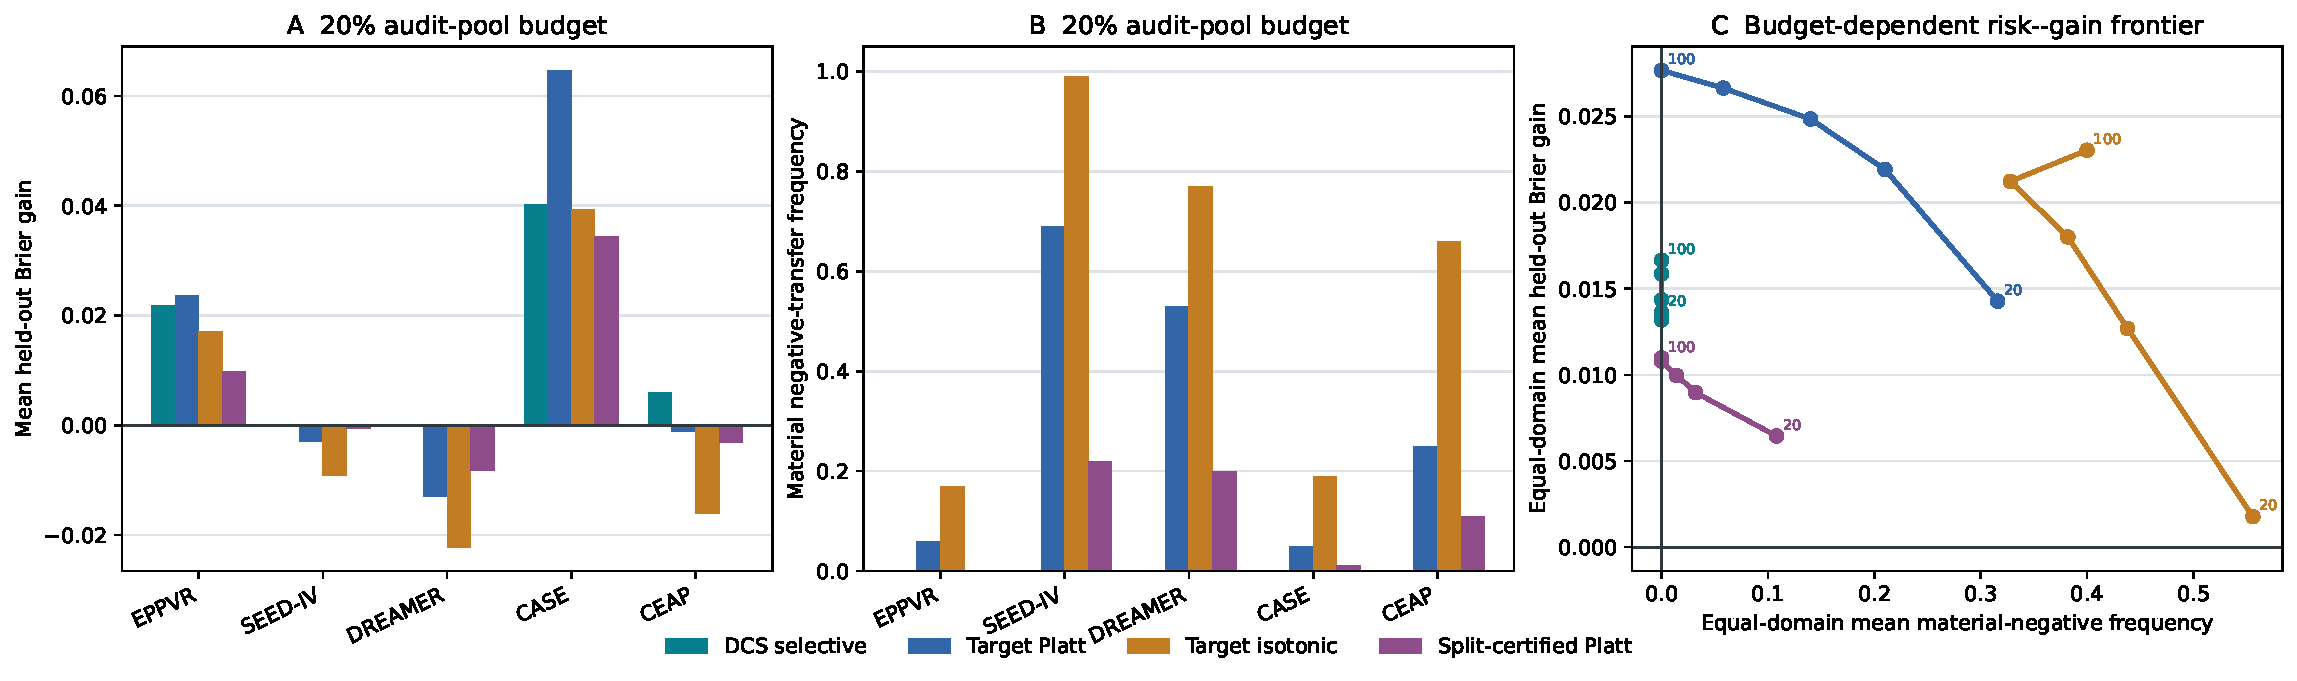
\includegraphics[width=\textwidth]{figures/fig_budget_risk_gain_tradeoff.pdf}
\caption{Retrospective audit-budget tradeoff on the fixed v11 held-out halves. (A) Mean held-out Brier gain at 20\% of the audit-pool budget. (B) Material-negative-transfer frequency at the same budget; identity fallback is a non-intervention and is not counted as effectiveness. (C) Equal-domain descriptive mean gain versus material-negative frequency across the five tested budgets; numeric annotations are percentages of the fixed audit pool. Panel C is a sensitivity summary, not a population-weighted or prospective external estimate.}
\label{fig:budget-tradeoff}
\end{figure*}

\begin{table*}[t]
\centering
\caption{Minimum- and full-budget comparison of selective DCS-OPCT and direct target Platt scaling over 100 audit repetitions. Gain is evaluated on the same fixed held-out half. Material negative denotes a released action with Brier gain below $-0.001$.}
\label{tab:budget-core}
\small
\setlength{\tabcolsep}{3pt}
\begin{tabular}{llrrrrrr}
\toprule
Dataset & Budget & $n_L$ & \multicolumn{3}{c}{DCS-OPCT} & \multicolumn{2}{c}{Target Platt} \\
\hline
 & & & Release (\%) & Gain & MNT (\%) & Gain & MNT (\%) \\
\midrule
EPPVR & Minimum & 32 & 83 & 0.0218 & 0 & 0.0237 & 6 \\
EPPVR & Full & 160 & 100 & 0.0263 & 0 & 0.0366 & 0 \\
SEED-IV & Minimum & 24 & 0 & 0.0000 & 0 & -0.0030 & 69 \\
SEED-IV & Full & 120 & 0 & 0.0000 & 0 & -0.0001 & 0 \\
DREAMER & Minimum & 24 & 0 & 0.0000 & 0 & -0.0129 & 53 \\
DREAMER & Full & 120 & 0 & 0.0000 & 0 & 0.0061 & 0 \\
CASE & Minimum & 32 & 83 & 0.0402 & 0 & 0.0647 & 5 \\
CASE & Full & 160 & 100 & 0.0485 & 0 & 0.0826 & 0 \\
CEAP & Minimum & 32 & 71 & 0.0060 & 0 & -0.0011 & 25 \\
CEAP & Full & 160 & 100 & 0.0085 & 0 & 0.0132 & 0 \\
\bottomrule
\end{tabular}

\end{table*}

\subsection{Fixed support gates rejected unsupported domains}

SEED-IV failed the component displacement gate: the absolute probability mean shifts were 0.159 for CORAL and 0.364 for quantile mapping, both above 0.10. DREAMER passed the individual shift budgets but failed the witness, with directional agreement 0.838 and normalized disagreement 0.371. The action was therefore set to identity in both datasets before audit outcomes could support release. Figure~\ref{fig:support} shows how the component and witness criteria separated released and rejected actions.

\begin{table}[t]
\centering
\caption{Unlabeled applicability diagnostics. Shift columns report absolute mean probability displacement.}
\label{tab:applicability}
\small
\begin{tabular}{lrrrrrl}
\toprule
Dataset & CORAL & Quantile & Agree. & Cosine & Disagree. & Gate \\
\midrule
EPPVR & 0.055 & 0.046 & 0.938 & 0.997 & 0.209 & Pass \\
CASE & 0.060 & 0.053 & 0.994 & 1.000 & 0.080 & Pass \\
CEAP & 0.037 & 0.044 & 0.925 & 0.947 & 0.208 & Pass \\
SEED-IV & 0.159 & 0.364 & -- & -- & -- & Fail \\
DREAMER & 0.022 & 0.035 & 0.838 & 0.977 & 0.371 & Fail \\
AVDOS-VR & 0.151 & 0.370 & -- & -- & -- & Fail \\
FACED & 0.122 & 0.334 & -- & -- & -- & Fail \\
\bottomrule
\end{tabular}
\end{table}

\begin{figure}[t]
\centering
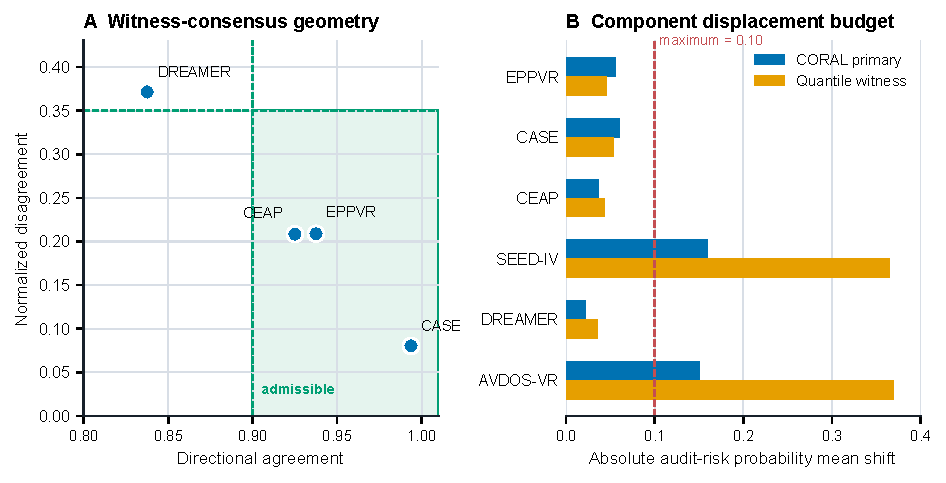
\includegraphics[width=\textwidth]{figures/fig_v11_support_gate_geometry.pdf}
\caption{Unlabeled support-gate geometry. Component probability-displacement limits are evaluated before witness agreement. Dashed boundaries indicate the frozen release thresholds. Domains outside any required boundary return the identity probability.}
\label{fig:support}
\end{figure}

A frozen leave-one-component diagnostic separated early screening from final release control. Removing only the quantile witness sent DREAMER to the labeled audit, where its Brier gain was $-0.0005$ and the 95\% lower certificate bound was $-0.0041$; the certificate rejected release. Removing the complete unlabeled applicability screen additionally sent SEED-IV to audit, where the gain was $-0.0315$ and the lower bound was $-0.0446$; release was again rejected. Thus the screen and witness saved labels by rejecting unsupported candidates before outcome access, whereas the certificate supplied the final veto in these observed domains. Replacing the distribution-covered assignment with the 100 already stored random balanced half-audits reduced CEAP's certification rate from the deterministic v11 pass to 0.60. No threshold, seed, candidate probability, or held-out row was changed for this diagnostic (Supplementary Material).

Under the common 720-configuration ceiling, certificate-only processing sent all 720 labels to action-stage certification, the single-gate variant used 600, and full DCS-OPCT used 480. The three calibration variants preserved the same observed release set---EPPVR, CASE, and CEAP---and the same equal-domain mean held-out Brier gain of 0.01665. Thus, the complete unlabeled sequence reduced retrospective action-stage label demand by 33.3\% relative to certificate-only processing without changing the archived release set. This is a same-assignment efficiency diagnostic, not proof that either gate is prospectively necessary; its complete figure and table are reported in the Supplementary Material.

Every tested one-at-a-time relaxation preserved identity in the unsupported development and external domains. Only the strictest settings changed an action, affecting EPPVR through directional agreement and CEAP through directional agreement, displacement cosine, or the Brier lower-bound certificate. Across 6,561 joint local scenarios, only three release patterns occurred, all subsets of the frozen EPPVR--CASE--CEAP set. Full margins and a worked EPPVR/EEGEmotions-27 trace are reported in the Supplementary Material.

\subsection{External tests defined applicability and endpoint boundaries rather than effectiveness confirmation}

All four completed external stress tests stopped before a released labeled correction. In the post-access AVDOS-VR PPG analysis, participant identity was decodable, but dose effects were heterogeneous and both probability shifts (0.151 and 0.370) exceeded the frozen 0.10 applicability budget. In the post-access FACED common-montage analysis, participant identity was strongly decodable (balanced accuracy 0.885--0.992), yet dose-induced amplification remained between $-0.0166$ and 0.0139 and no configuration reached the 0.02 endpoint. Its probability shifts (0.122 and 0.334) also exceeded the applicability budget, and the event-free endpoint made discrimination and calibration effectiveness non-estimable.

The separately locked pre-signal EEGEmotions-27 test likewise stopped at the unlabeled component screen. CORAL and quantile probability displacements were 0.1073 and 0.1281, respectively, although both maps preserved rank with zero inversions. No category-polarity outcome entered action selection and no labeled release certificate was attempted. Post-hoc inspection found weak dual-unseen category-polarity performance, non-monotonic dose behavior, ranking reversals, and negative held-out gains for the rejected counterfactual maps; these observations characterize the failure boundary but did not determine it.

The EKM-ED attempt failed one stage earlier under a stronger prospective information boundary. All 47 questionnaire participants were attempted after the schema-bound implementation lock. Of 188 possible participant--film units, 10 lacked a registered clean signal file, 45 had no complete finite registered key-moment window, and 47 had only one; 86 trials retained all three windows. After excluding six valence and 14 arousal midpoint ratings, no participant in either task satisfied the frozen requirement of at least three retained trials and both classes. The minimum 30-participant gate therefore failed, no pre-outcome design or unlabeled action was locked, and no emotion model, material event, calibration candidate, or effectiveness outcome was fitted. This result directly shows that a public semantic key-moment specification need not yield a transportable configuration-level endpoint under a strict completeness contract.

These datasets therefore extend the tested applicability and endpoint-construction envelope and support the distinction between identity encoding, endpoint availability, and material utilization. They do not confirm calibration effectiveness, future-domain non-harm, or population safety. Full protocol histories, figures, tables, immutable action traces, and the EKM-ED structural-failure record are provided in the Supplementary Material.

\section{Discussion}
\label{sec:discussion}

\subsection{A closed loop from mechanism to audit action}

The principal contribution is not any single transformation. Its strongest positive transport evidence is the EPPVR release that remained beneficial after configuration-level covariate holdout and raw test-participant separation; the broader three-domain transductive release set is development evidence. The fully participant- and training-row-disjoint EPPVR analysis did not release a correction because its audit-side probability displacement exceeded the frozen applicability limit. This result places a sharper upper bound on the claim: DCS-OPCT exhibited a positive conditional release under partial independence and fail-closed behavior under complete within-dataset population separation, but no positive fully training-data-independent release. The study connects three questions that are usually evaluated separately. The counterfactual dose experiment asks whether controlled identity opportunity changes apparent performance. The ranking analysis asks whether that change matters for model selection. The frozen risk model turns this consequence into an auditable event, and DCS-OPCT addresses the observed failure of its probabilities under domain shift. A probe alone cannot establish utilization, a risk score without calibration cannot support probability-based allocation, and a calibrator without a mechanism-derived endpoint becomes an unmotivated adapter comparison. The observed division of labor among stages comes from retrospective leave-one-component diagnostics and is not a prospective necessity theorem.

The dose results also clarify why shortcut risk should not be reduced to identity decodability. Participant identity was often recoverable, but utilization varied across configurations and was not generally monotonic with dose. Encoding supplies the capacity for a shortcut, while identity--label opportunity supplies a potential benefit; the emotion model still has to use their interaction. This distinction explains why the risk model includes opportunity, encoding, and their interaction rather than an identity-probe score alone.

\subsection{What is transported, and what is not}

DCS-OPCT does not transform EEG trials for emotion recognition and does not update an emotion classifier. It calibrates the probability that an evaluation configuration will exhibit at least 0.02 dose-induced optimism. The intended user is therefore a benchmark designer or model evaluator deciding which configurations require a stricter identity audit, not a clinical system assigning an emotional state to a patient.

This narrower endpoint is also why preserving order is valuable. EPPVR showed that the frozen score retained ranking information while overpredicting absolute risk. A positive-slope map can correct probability levels without changing audit priority. The zero AUROC difference is a mathematical consequence of verified monotonicity, not an empirical claim that discrimination improved. Brier gain supplies the relevant effectiveness endpoint because it rewards accurate probabilities and penalizes confident errors \cite{brier1950verification}.

\subsection{Selective release and bounded non-harm evidence}

The evaluated risk-control logic has two components. For an eligible action, a fixed labeled audit had to provide a positive lower-bound certificate before held-out release. For an ineligible action, the method made no change. Across 100 repeated nested audits at each of five budgets, no DCS-OPCT release produced material negative transfer. This was not reproduced by direct Platt, beta, temperature, or isotonic calibration at low budgets, and split-fit/certified and same-audit cross-fit-certified Platt and beta maps still released harmful corrections in several domains. The comparison supports the engineering value of coupling an unlabeled applicability screen, a precomputed order-preserving candidate, and a limited-label release certificate. It does not establish a universal guarantee: even with zero observed DCS events, the one-sided 95\% upper bound among released actions ranged from 2.95\% to 4.64\% across domain--budget cells with releases. A future domain can also violate the assumptions represented by the component, witness, audit geometry, or finite certificate.

The leave-one-component diagnostic further indicates a division of labor rather than interchangeable safeguards. The quantile witness and the broader applicability screen did not improve the held-out gain of the three already supported domains; instead, they prevented DREAMER and SEED-IV from consuming labeled audit capacity. When those early gates were removed, the unchanged certificate still blocked both candidates. Conversely, random balanced half-audits made the weak CEAP benefit inconsistently certifiable, whereas the outcome-blind distribution-covered assignment passed it with positive held-out gain. These are retrospective observations from the frozen domains, not proof that every component is necessary in every future domain. The same-ceiling reconstruction sharpened this interpretation: the unlabeled sequence saved 240 action-stage labels relative to certificate-only processing while preserving the archived release set, but it does not identify a prospective causal contribution or guarantee the same saving under a new target distribution.

Identity fallback deserves equally careful interpretation. It prevents the proposed correction from worsening the frozen probabilities because nothing is changed, but zero change is not evidence that the original probabilities are well calibrated. SEED-IV, DREAMER, AVDOS-VR, and FACED therefore support selective non-intervention, not successful adaptation. FACED further shows that an event-free endpoint does not demonstrate safety: without positive and negative endpoint instances, discrimination and probability calibration cannot be estimated. Treating abstention or non-estimability as effectiveness would erase the distinction on which the method is built. EEGEmotions-27 sharpened this boundary because the action failed on unlabeled probability displacement before category-polarity labels entered selection. Its identity result therefore demonstrates protocol adherence under an independently collected wearable-EEG geometry, not external calibration benefit. EKM-ED sharpens a still earlier boundary: when the frozen trial endpoint is structurally unavailable, even an identity fallback is never defined, and the only admissible result is non-estimability.

\subsection{Why distribution-covered auditing matters}

Earlier method versions revealed that the audit partition itself can determine whether a weak but real calibration benefit is detected. Random balanced half-audits were stable for EPPVR and CASE but released CEAP inconsistently. Increasing correction strength caused negative transfer. DCS-OPCT therefore left the probability action unchanged and improved how a fixed label budget represented the unlabeled target distribution. The geometry objective is not fitted to outcomes and cannot guarantee a representative sample in every relevant latent dimension, but it makes the audit allocation explicit, deterministic, and testable.

The framework is best viewed as limited-label target validation rather than fully unsupervised domain adaptation. Target labels are required for the certificate, but only after the candidate action and audit assignment have been locked from unlabeled information. This design fits settings in which a modest validation budget is available but unrestricted model redevelopment is not. The budget curves sharpen that use case: direct Platt and beta calibration became more effective as labels accumulated, whereas DCS-OPCT traded some attainable gain for fewer erroneous interventions at the smallest budgets. DCS-OPCT should therefore not replace ordinary recalibration when a large, representative labeled target set is available.

\subsection{Implications for EEG emotion-recognition studies}

The results support reporting evaluation protocols by deployment identity rather than by generic cross-validation terminology. A model intended for unseen users should be ranked under subject-disjoint or joint-disjoint conditions. When historical studies or operational constraints require overlapping evaluation, the proposed mechanism experiment can quantify how much model selection depends on identity opportunity. The audit-risk score then prioritizes configurations for closer inspection, while DCS-OPCT addresses cross-domain probability mismatch only when its release conditions are met.

The model-ranking analysis is particularly relevant for engineering comparisons. Differences of two balanced-accuracy points can change a selected representation or classifier even when they appear modest in isolation: 85\% of the evaluated joint-unseen selection units had a top-two margin at or below this level. The observed subject-exposure regrets in DEAP and MAHNOB-HCI were also of this order. Consequently, identity exposure is not only a reporting issue; it can redirect subsequent development toward a model that is inferior under the intended deployment split. Risk ordering concentrated material-event burden under restricted budgets, although the binary policy's advantage was confined to a bounded range of hypothetical relative costs.

\subsection{Limitations and required confirmation}

Several limitations bound the conclusions. First, the primary risk model was trained on only two public EEG datasets. A post-hoc seven-domain refit retained positive mechanism directions and improved pooled probability error, but it failed its prespecified leave-dataset-out discrimination and operating-point gate. Because those additional domains had already been inspected during method development, this analysis diagnoses persistent domain heterogeneity rather than providing independent validation or replacing the frozen model. Second, DCS-OPCT v11 was developed retrospectively after multiple predecessor methods were evaluated. Preserving all failures improves transparency but does not turn the final development evidence into prospective confirmation. Third, the material-event threshold of 0.02 is operational rather than physiological. A post-hoc 0.01--0.03 analysis located it within, and at the lower edge of, the tested range that retained cross-dataset discrimination, probability skill, and operating-point performance with adequate event counts. Crossed test-sample resampling nevertheless showed that almost every source configuration had an amplification interval spanning 0.02 and that no lower-confidence-bound event remained. Probabilistic relabeling preserved positive soft-label gains for the two inductively released actions but weakened hard-label discrimination and coefficient stability. The frozen event is therefore retained for protocol continuity, not treated as a precisely observed biological state. Candidate-margin and audit-utility analyses showed engineering relevance but reused the same development experiments and hypothetical costs. They support operational interpretation only and cannot establish a clinically meaningful cutoff, measured cost effectiveness, or threshold optimality. The local action-stability grid likewise describes the neighborhood of the frozen decisions; because it was conducted after observing the development results, it cannot validate or optimize any threshold.

Fourth, the primary held-out evaluation was transductive with respect to target covariates and repeatedly reused the same frozen halves. The covariate-unseen sensitivity retained positive releases for EPPVR and CASE but not CEAP. After endpoint reconstruction on disjoint raw test groups, only EPPVR remained certified; CASE returned the original probability. The final EPPVR raw-partition-first sensitivity eliminated shared participants, raw rows, emotion-model training rows, identity-probe training rows, and fitted target-domain models, but its two component shifts exceeded the frozen applicability limit and no correction was released. This single 15/15 split therefore resolves the most direct within-dataset training-overlap objection while simultaneously showing that the positive EPPVR action is not robust to full population separation. It remains a retrospective sensitivity from the same dataset, not an independent external confidence interval or estimate of future-domain risk; the other four domains were not rebuilt under this expensive protocol. Direct Platt and beta calibration outperformed DCS-OPCT at the full budget in four domains, so no general calibration-superiority claim is supported. Fifth, the CORAL and quantile components align only selected aspects of the mechanism-feature distribution. Their agreement is a safeguard, not proof of causal invariance. Sixth, the current endpoint concerns subject-axis material optimism. A stimulus-axis model requires a verified shared physical-stimulus map and separate validation.

The EPPVR raw and processing chain verified 30 participants, 14 trials per participant, ten synchronized channels, 100-Hz sampling, FP1/FP2 as channels 0/1, and a 10-s per-trial baseline followed by 60 s of post-baseline data. Author-supplied acquisition records identify a DPVR E4 head-mounted display and an ADS1299-based EEG acquisition front end, with both reference and ground electrodes placed at the right ear. Channels 5--9 collectively comprise two EOG channels, one PPG channel, one GSR channel, and one temperature channel; their exact within-block order could not be recovered from the inspected acquisition and analysis records. The third label column is the participant-rated dominance dimension. Neither channels 5--9 nor dominance enters the present analysis. The protocol was approved by the Ethical Committee of the University of Electronic Science and Technology of China (approval no. 106142023122227999); written informed consent and authorization for secondary analysis were obtained.

Finally, no external attempt completed a successful registered effectiveness test. AVDOS-VR required post-access amendments to its label semantics, quality handling, and participant-level trial structure. FACED failed its registered 32-channel eligibility rule because two acquisition montages shared only 30 comparable EEG channels; the amended common-montage analysis then contained no material event at the frozen endpoint. Both completed analyses are therefore exploratory. EEGEmotions-27 was locked before signal and outcome access after repository metadata disclosure, but both unlabeled projections were inapplicable; it supplies a separately tested failure boundary rather than effective external release. EKM-ED met the prospective reservation, checksum, header-only schema, implementation-lock, and no-retuning requirements, but failed the frozen trial-completeness and participant-eligibility gate before model fitting. This is stronger evidence of procedural integrity and endpoint fragility, not evidence of calibration effectiveness. A future positive external claim still requires a compatible prospectively reserved dataset with sufficient endpoint variation and a non-identity action that passes the unchanged audit and held-out gates. Until such a test succeeds, the strongest admissible conclusion is selective development-domain calibration with observed abstention and non-estimability boundaries.

\section{Conclusion}

Identity exposure in repeated-measures affective data can alter apparent performance and reverse model selection, but its effect cannot be inferred from identity decodability alone. We linked a counterfactual identity-dose experiment to a mechanism-derived audit-risk model and then addressed the model's cross-domain calibration failure with DCS-OPCT. The original transductive analysis improved outcome-held-out Brier score in EPPVR, CASE, and CEAP; excluding held-out covariates retained EPPVR and CASE, whereas additional raw test-group separation retained only EPPVR. When EPPVR was rebuilt from two fully disjoint 15-participant training populations, the frozen applicability screen stopped the correction before outcome-based release. In the prospectively locked EKM-ED attempt, the frozen key-moment endpoint itself failed structural eligibility before model fitting. Endpoint resampling also showed substantial uncertainty around the 0.02 binary event. No material negative transfer was observed for released actions, but zero observed events, return-original decisions, and structurally unavailable endpoints provide bounded evidence rather than proof of safety. These findings support selective configuration-level audit-risk calibration only within evaluated development support while directly demonstrating target-batch, endpoint, and underlying-data dependence. They do not establish a positive fully training-data-independent release, universal transport safety, successful prospective external effectiveness, or direct improvement of EEG emotion classification.

\section*{Data and code availability}


A checksum-verified reproducibility package, source code, aggregate outputs, and validation reports are publicly available at \url{https://github.com/dohonwei/dsc-opct}. DEAP, MAHNOB-HCI, CASE, CEAP, SEED-IV, DREAMER, AVDOS-VR, FACED, EEGEmotions-27, and EKM-ED remain subject to their original access conditions. The EKM-ED source archive is openly available under CC BY 4.0 at DOI 10.5281/zenodo.8431451; the package records its official checksum, schema receipts, implementation lock, and structural-failure audit rather than redistributing the 4.35-GB archive. The package contains deterministic experiment scripts, GPU settings, split and audit assignments, row-level prediction outputs where licensing permits, frozen-model checksums, failure records, summary tables, figures, and independent validation reports. A dataset-level availability matrix states the role, access route, releasable derivatives, and inferential boundary for every completed and prospectively reserved dataset. Public release of derived data will follow source-dataset licenses, data-use agreements, institutional approval, and participant-consent restrictions; restricted participant-level source data are not included.

\section*{Ethics statement}

The EPPVR data-collection protocol was reviewed and approved by the Ethical Committee of the University of Electronic Science and Technology of China (approval no. 106142023122227999). Written informed consent was obtained from all participants, and authorization covered the secondary analysis reported in this study. All other datasets were analyzed under their original access, ethics, and participant-consent conditions.

\section*{Declaration of competing interest}

The authors declare that they have no known competing financial interests or personal relationships that could have appeared to influence the work reported in this paper.

\section*{Funding}

This work was supported by the National Natural Science Foundation of China (No. 62172081).

\bibliographystyle{elsarticle-num}
\bibliography{dcs_opct_v11_bspc_refs}

\end{document}
